% DO NOT COMPILE THIS FILE DIRECTLY!
% This is included by the other .tex files.

\begin{frame}
\titlepage
\end{frame}

\begin{frame}
\frametitle{What is MISP?}
\begin{itemize}
       \item MISP is a {\bf threat information sharing} platform that is free \& open source software
       \item A tool that {\bf collects} information from partners, your analysts, your tools, feeds
       \item Normalises, {\bf correlates}, {\bf enriches} the data
       \item Allows teams and communities to {\bf collaborate}
       \item {\bf Feeds} automated protective tools and analyst tools with the output
       \item MISP is a complete threat intelligence platform with strong sharing capabilities and extendability
\end{itemize}
\end{frame}


\begin{frame}
  \frametitle{The aim of this presentation}
  \begin{itemize}
     \item A small update on the state of MISP's ongoing development
     \item Some highlights of the changes that were introduced
     \item Upcoming changes
     \item Cerebrate (a MISP companion) update
     \item Workflows
  \end{itemize}
\end{frame}

\begin{frame}
  \frametitle{MISP's evolution since past 6 months}
  \begin{itemize}
    \item 9 releases
    \item 1775 commits
    \item 74 contributors contributing to the core software and its components
  \end{itemize}
\end{frame}

\begin{frame}
  \frametitle{Main focus was securing our data and tooling}
  \begin{itemize}
      \item Current {\bf geo-political situation} lead to new challenges
      \item It has been an interesting time period with quite some activity
      \item Our goal was to {\bf shore up the security} aspects of MISP and Cerebrate
      \item Build new functionalities and tools to allow users to {\bf protect their data}
  \end{itemize}
\end{frame}

\begin{frame}
  \frametitle{Sharing group blueprints}
  \begin{itemize}
     \item Solving the issue of {\bf sharing group lifecycle management}
     \item Build SG blueprints for reusable, maintainable sharing groups
     \item Abstract sharing groups, organisation metadata as building blocks
     \item Solve newly arising sharing challenges
  \end{itemize}
\end{frame}

\begin{frame}
\frametitle{Sharing group blueprints}
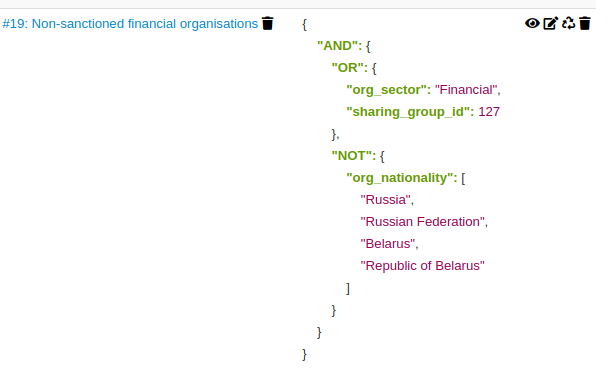
\includegraphics[scale=0.6]{images/blueprints2.png}
\end{frame}

\begin{frame}
  \frametitle{Cryptographic signing and tamper protection}
  \begin{itemize}
     \item Need to be able to share and ensure the {\bf veracity of critical events}
     \item Tampering by {\bf malicious intermediaries}, even in closed networks became a new fear
     \item We came up with a solution that allows us to {\bf lock down critical events}
     \item Limits the distribution, but {\bf increases the resilience} of MISP immensely
  \end{itemize}
\end{frame}

\begin{frame}
\frametitle{Cryptographic signing and tamper protection}
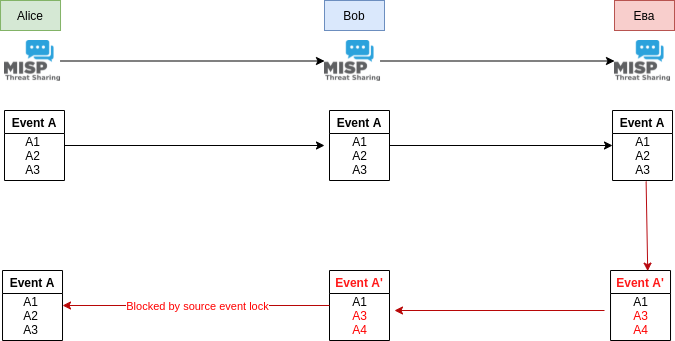
\includegraphics[scale=0.5]{images/signing1.png}
\end{frame}

\begin{frame}
\frametitle{Cryptographic signing and tamper protection}
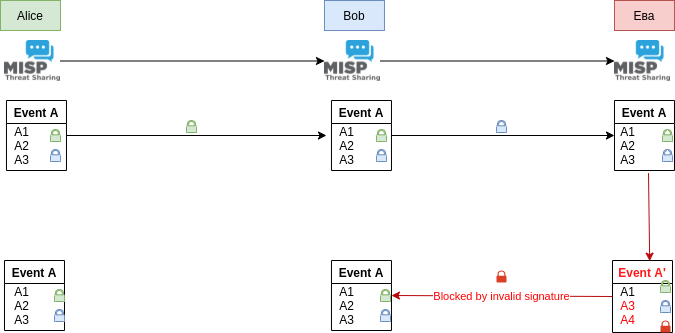
\includegraphics[scale=0.5]{images/signing2.png}
\end{frame}

\begin{frame}
\frametitle{Cryptographic signing and tamper protection}
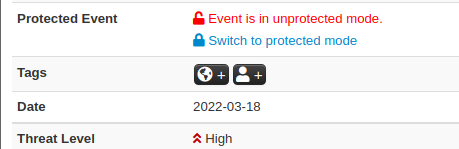
\includegraphics[scale=0.6]{images/signing3.png}
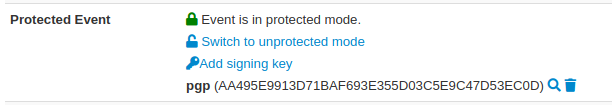
\includegraphics[scale=0.6]{images/signing4.png}
\end{frame}

\begin{frame}
  \frametitle{Other major improvements}
  \begin{itemize}
      \item Various other new functionalities that improve our day to day use of the tool
  \end{itemize}
\end{frame}

\begin{frame}
  \frametitle{Long list of security fixes}
  \begin{itemize}
      \item Partially from user reports
      \item Partially by an exhaustive pentest series
      \item Massive thank you to {\bf Zigrin Security} for conducting the tests...
      \item ...and to the {\bf Luxembourgish Army} for financing it
      \item Multiple {\bf CVEs} resolved, including a {\bf critical one that required a silent release}
      \item Make sure you stay up to date!
  \end{itemize}
\end{frame}

\begin{frame}
\frametitle{Long list of security fixes}
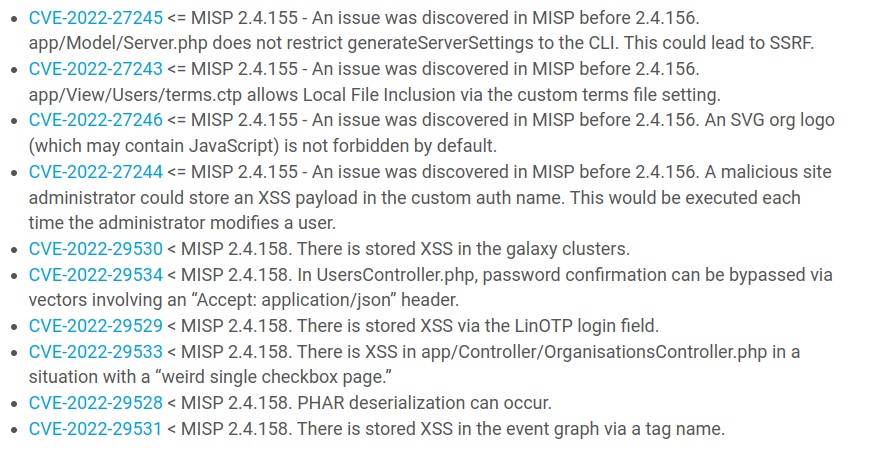
\includegraphics[scale=0.4]{images/security.png}
\end{frame}


\begin{frame}
  \frametitle{Event warning system}
  \begin{itemize}
     \item Build a rule based tool that analyses an event and {\bf recommends improvements}
     \item Typical issues easily caught (missing TLP, lack of context, etc)
     \item Simple to extend, flexible
  \end{itemize}
\end{frame}

\begin{frame}
\frametitle{Event warning system}
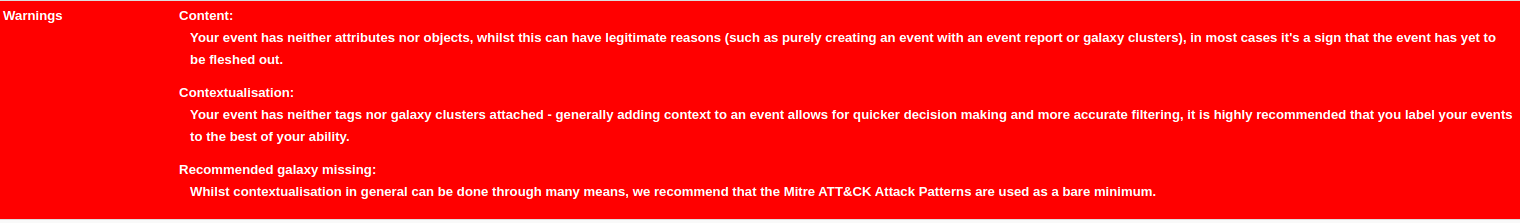
\includegraphics[scale=0.3]{images/warnings.png}
\end{frame}


\begin{frame}
  \frametitle{Massive rework of the STIX integrations}
  \begin{itemize}
     \item Our resident STIX guru (Christian Studer) has become {\bf co-chair of the STIX commitee} at OASIS
     \item Massive rework of how we handle {\bf STIX ingestion / generation}
     \item Continuous work with {\bf MITRE/CISA} to improve the integration
     \item STIX subsystem spun off as a standalone system {\bf misp-stix}\footnote{\url{https://github.com/MISP/misp-stix}}
     \item Can be used a standalone to convert in both directions MISP standard format to all the STIX variantes
  \end{itemize}
\end{frame}

\begin{frame}
  \frametitle{Further synchronisation filtering methods}
  \begin{itemize}
     \item The ability to {\bf exclude} certain attribute {\bf types from the synchronisation}
     \item Comes with some risks, but solves some issues
     \item An example: {\bf Exclusion of malware samples when sharing towards classified networks}
  \end{itemize}
\end{frame}

\begin{frame}
  \frametitle{Advanced timelining}
  \begin{itemize}
     \item Rework of the timelining in MISP
     \item Inclusion of images, sightings
     \item Various other improvements
  \end{itemize}
\end{frame}

\begin{frame}
\frametitle{Timelining}
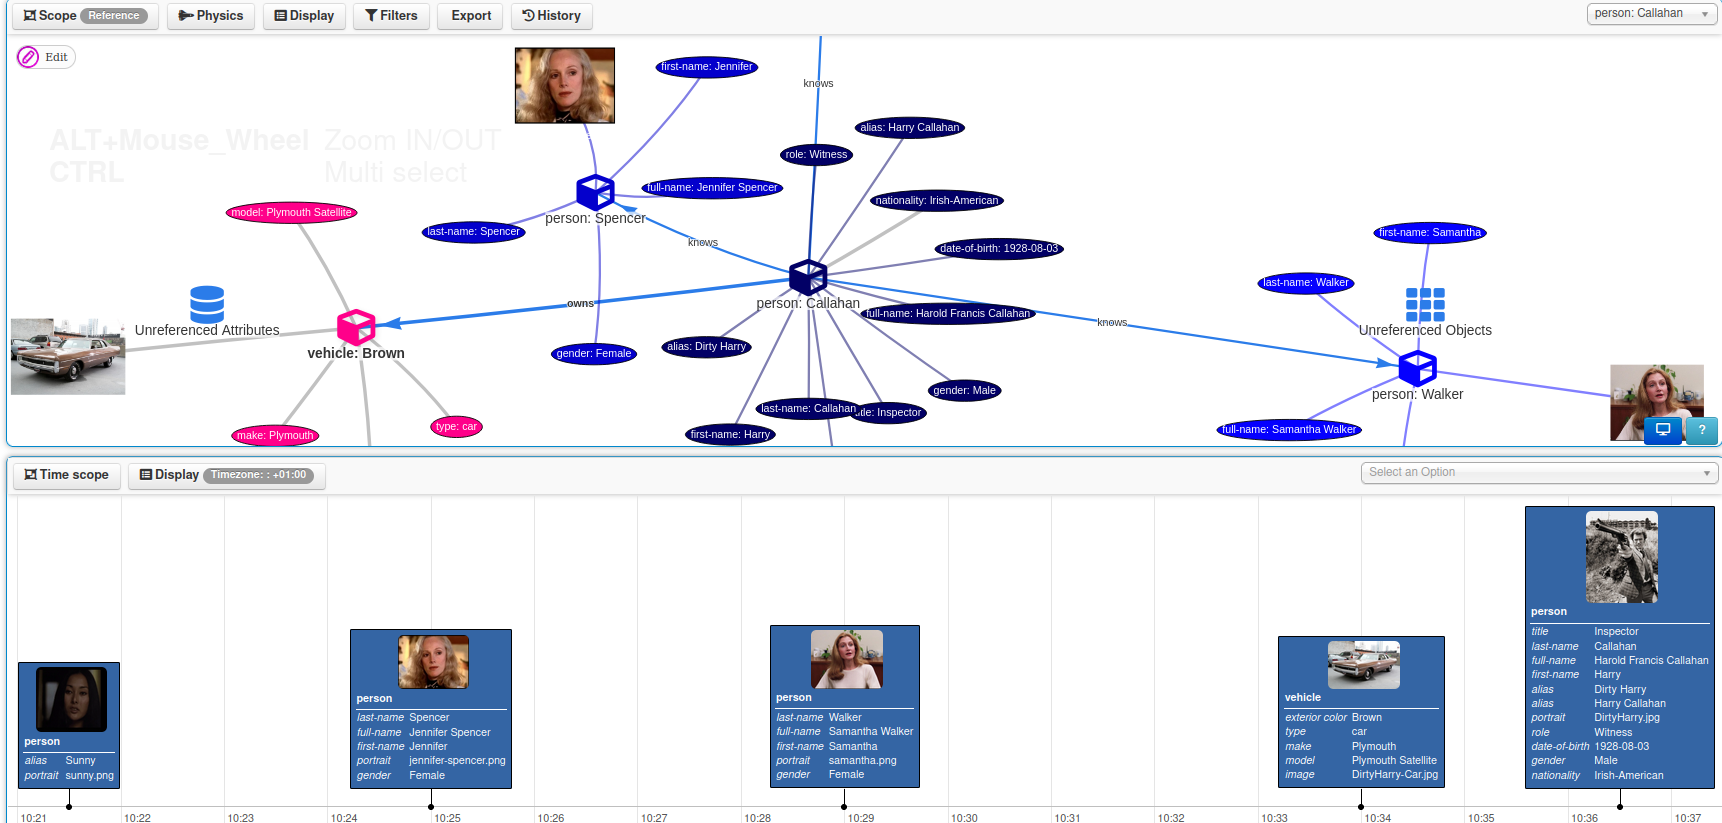
\includegraphics[scale=0.2]{images/timelining.png}
\end{frame}

\begin{frame}
  \frametitle{New background processor}
  \begin{itemize}
     \item Since late November last year we have had a {\bf new background processing engine}
     \item Fully optional for now
     \item Lean, closer to an OS native implementation via {\bf Supervisor}
     \item Gets rid of a lot of the baggage of our previous system (scheduling)
     \item Implemetation by @righel (Luciano Righetti)
  \end{itemize}
\end{frame}


\begin{frame}
  \frametitle{Long list of other fixes}
  \begin{itemize}
     \item Usability fixes
     \item Performance improvements
     \item Bug fixes
     \item Too many improvements to the galaxies, taxonomies, object templates to list!
     \item Huge thank you to {\bf Jakub Onderka} for the {\bf constant stream of improvements}
  \end{itemize}
\end{frame}

\begin{frame}
  \frametitle{Workflows in MISP}
  \begin{itemize}
     \item Outcome of our initial work from GeekWeek 7.5\footnote{\href{https://cyber.gc.ca/en/events/geekweek-75}{Workshop organized by the Canadian Cyber Center}}
     \item Goal: Modifying the execution of certain {\bf core functionalities}
     \item Basically a {\bf hooking mechanism}
     \item Modular approach using {\bf MISP-modules} or {\bf PHP modules}
     \item Build and execute admin defined tasks on various actions
     \item Modify data in place, block, fire-and-forget
     \item All exposed via a {\bf completely new GUI}
  \end{itemize}
\end{frame}

\begin{frame}
  \frametitle{Workflows in MISP}
  \begin{itemize}
     \item {\bf Branching} codebase
     \item Context sensitive, per-module filters
     \item Implemented by our UI expert Sami "GraphMan" Mokaddem 
  \end{itemize}
\end{frame}


\begin{frame}
\frametitle{Workflows in MISP}
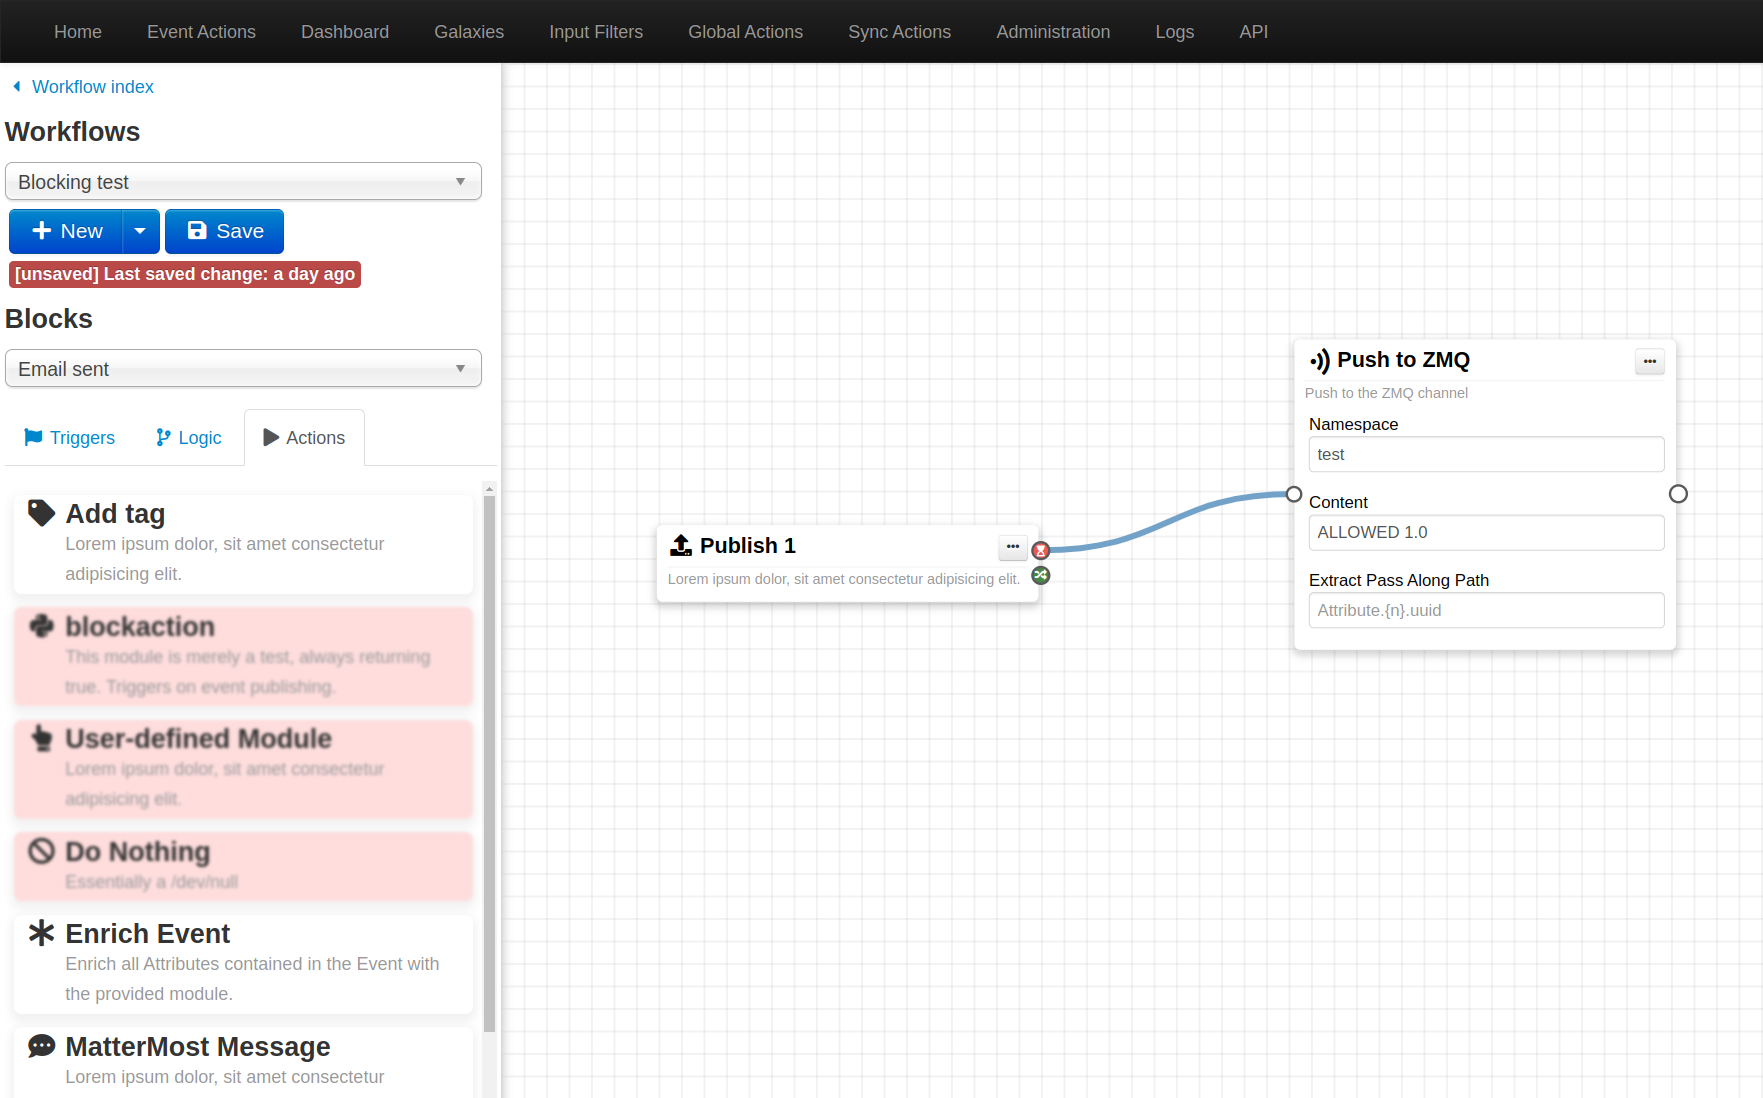
\includegraphics[scale=0.2]{images/workflows1.png}
\end{frame}

\begin{frame}
\frametitle{Workflows in MISP}
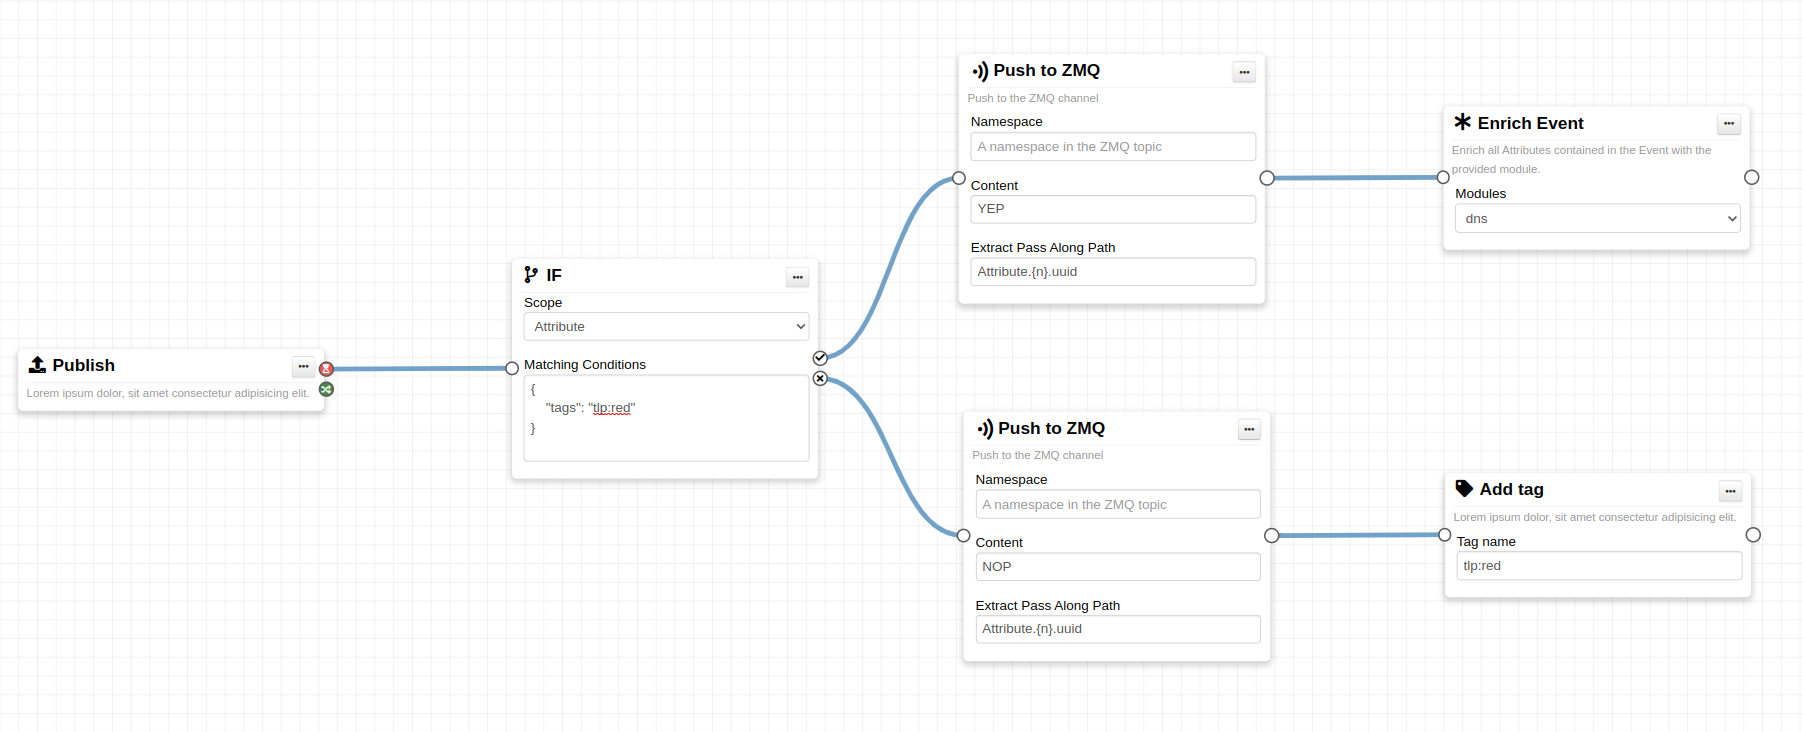
\includegraphics[scale=0.2]{images/workflows2.png}
\end{frame}


\begin{frame}
  \frametitle{External data guard}
  \begin{itemize}
     \item Work in {\bf collaboration with BICES}
     \item Proxy server\footnote{\url{https://github.com/MISP/misp-guard}} that {\bf inspects and blocks potential data leaks} during synchronisation
     \item Standalone
     \item Simplistic design and {\bf easy to audit}
     \item Modular {\bf rule based} system
  \end{itemize}
\end{frame}

\begin{frame}
  \frametitle{Various reworks to support STIX mappings}
  \begin{itemize}
     \item {\bf Relationships for tags/galaxies}
     \item {\bf Templating} for galaxy cluster creation
     \item Dot notation {\bf deep cluster elements}
     \item Built in {\bf TAXII 2.1 export support} with the help of MITRE/CISA
  \end{itemize}
\end{frame}

\begin{frame}
\frametitle{Quick Cerebrate update}
\begin{center}

\includegraphics[scale=0.4]{images/cerebrate.png}
\end{center}
\end{frame}

\begin{frame}
  \frametitle{Quick Cerebrate update}
  \begin{itemize}
     \item 5 new releases
     \item Deployment for the {\bf CSIRT network} ongoing
     \item A host of new functionalities to solve day to day issues we have in the CSIRT community
  \end{itemize}
\end{frame}

\begin{frame}
  \frametitle{User management}
  \begin{itemize}
     \item Reworked completely
     \item Tight integration with {\bf KeyCloak}
     \item Full user provisioning / maintaining via Cerebrate
  \end{itemize}
\end{frame}

\begin{frame}
  \frametitle{Reworked meta information system}
  \begin{itemize}
     \item Introduction of {\bf context specific custom fields}
     \item Custom {\bf search algorithms} (for example CIDR block lookups for constituency information)
     \item Customisable and {\bf blueprint-able data model}
  \end{itemize}
\end{frame}

\begin{frame}
  \frametitle{API along with its documentation fleshed out}
  \begin{itemize}
     \item {\bf OpenAPI integration} similarly to MISP
     \item Integration tests and introduction of a {\bf CI pipeline}
     \item Documentation and API examples available in Cerebrate directly
  \end{itemize}
\end{frame}

\begin{frame}
  \frametitle{Security fixes}
  \begin{itemize}
     \item Cerebrate, similarly to MISP received an in-depth pentest by {\bf Zigrin Security}
     \item Likewise funded by the {\bf Luxembourgish Army}
     \item Besides fixes to vulnerabilities, a host of usability findings and fixes
     \item {\bf 5 CVEs} published
     \item \url{https://www.cerebrate-project.org/security.html}
  \end{itemize}
\end{frame}

\begin{frame}
  \frametitle{Get in touch if you have any questions}
  \begin{itemize}
    \item Contact CIRCL
    \begin{itemize}
      \item info@circl.lu
      \item \url{https://twitter.com/circl_lu}
      \item \url{https://www.circl.lu/}
    \end{itemize}
    \item Contact MISPProject 
    \begin{itemize}
      \item \url{https://github.com/MISP}
      \item \url{https://gitter.im/MISP/MISP}
      \item \url{https://twitter.com/MISPProject}
    \end{itemize}
    \item Cerebrate project
    \begin{itemize}
      \item \url{https://github.com/cerebrate-project}
      \item \url{https://github.com/cerebrate-project/cerebrate}
    \end{itemize}
  \end{itemize}
\end{frame}
